\subsection{Simulation Evaluation}
In this section, we perform a numerical evaluation of our proposed method
with two goals: (1) confirms the scalability and (2) observe the behavior 
of the method as input parameters change. 
%
We implemented our proposed algorithms in C++. Dinic's algorithm is used to solve the max-flow problem \cite{dinitz1970algorithm} for simplicity. 
The methods are evaluated at an Intel\textsuperscript{\textregistered} Core\textsuperscript{TM} i5-10600K CPU at 4.1HZ.
%
For the three use cases (~\ref{fig:sc-sweep} (b)(c)(d)), we
programmatically create a large number of test cases, with up to 
$6,000$ randomly generated polygonal obstacles. 
%
The number of vertices of each polygon ranges from 3 to 50, making the total vertices up to 
$100,000+$. 
%
~\ref{fig:sc-cases} shows the largest problem instances for the experiments with 
around $100,000$ vertices.
\begin{figure}[ht]
    \centering
    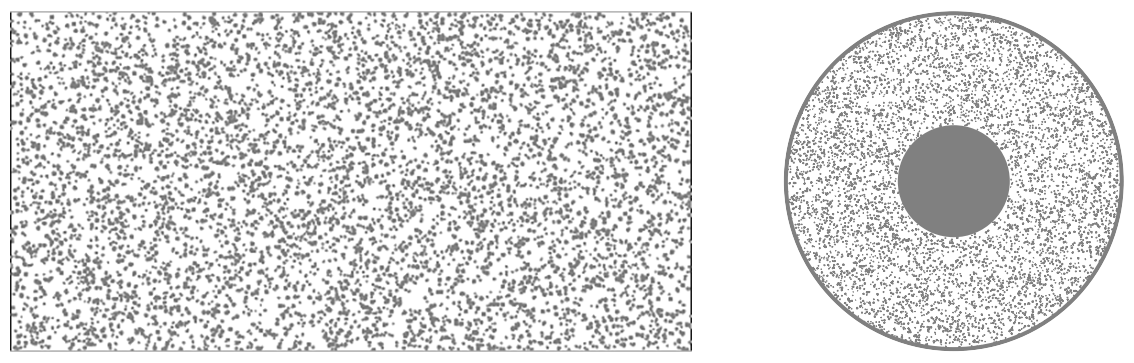
\includegraphics[width=.95\linewidth]{chapters/sc/fig/cases.png}
    \caption{Examples of programmatically generated test environments with total 
    vertices around $100,000$.}
    \label{fig:sc-cases}
\end{figure}

\textbf{Algorithm performance.} In a first set of evaluations, under an exponentially 
decaying sensing 
model, $\rho(r) = e^{-c\cdot r}$, we test the performance of our algorithm over 
the set of instances. Example allocation of robots along the sweep frontiers for 
the three cases are shown in ~\ref{fig:sc-sweep}(a) and ~\ref{fig:sc-simulations}. 
We limited the number of robots to be small so that the trajectories are more easily 
observed. It can be seen that the trajectories can vary significantly along the 
sweep frontiers for each case. 
% The first setting uses vertical sweep as the search schedule to sweep a rectangle.
% The second setting uses circular sweep, where guards are tasked to
% sweep $\mathcal{W}$ in a circular expansion manner.
% The thirst setting uses radial expansion as the search schedule, that is 
% a group of guards are tasked to sweep a circular regions in a radial rotational manner.
\begin{figure}[ht]
    \centering
    % 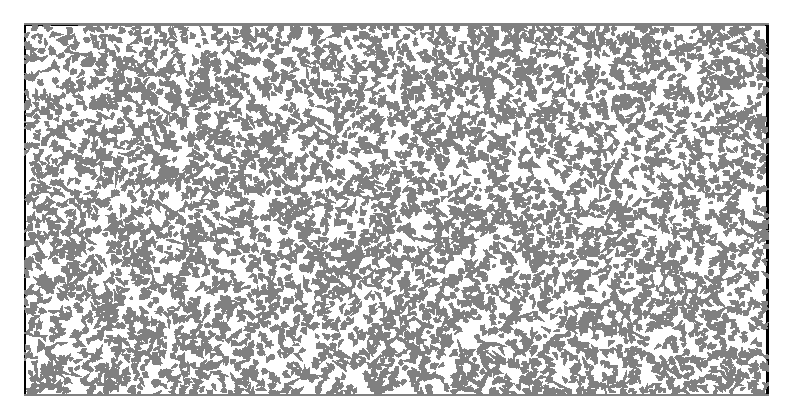
\includegraphics[width=.45\linewidth]{fig/vertical_large.eps}
    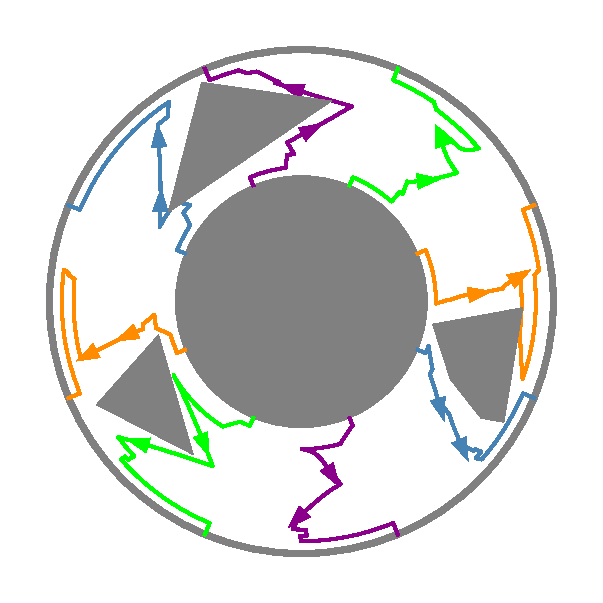
\includegraphics[width=.45\linewidth]{chapters/sc/fig/circular_sol.eps}\hspace{2mm}
    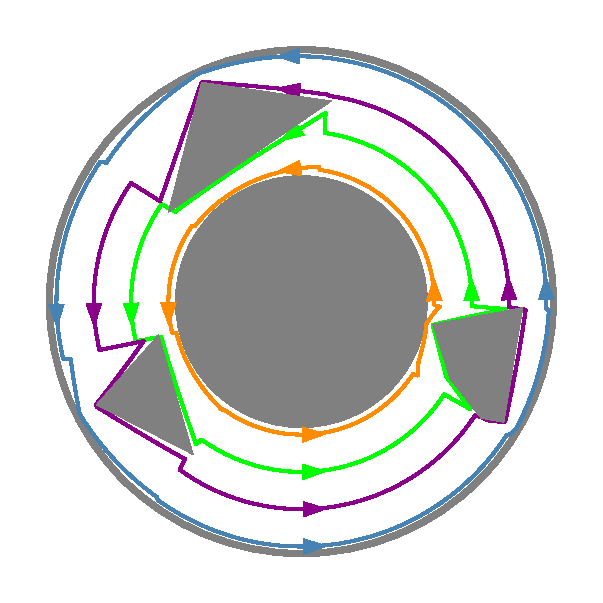
\includegraphics[width=.45\linewidth]{chapters/sc/fig/rotational_sol.eps}
    
    \caption[Example robot trajectories]{Example robot trajectories computed by our method for circular and radial 
    sweep use cases, respectively.
    }
    \label{fig:sc-simulations}
\end{figure}

In ~\ref{fig:sc-simulations_runtime}, the computational performance is thoroughly 
evaluated. As can be observed, our method scales fairly well, taking less than two seconds
to handle all cases, even those involving over $100,000$ vertices. 
%
%We show the running time information in ~\ref{fig:simulations_runtime}. 
%The algorithm scale up reasonably to $10^5$ vertices in around $1.5s$ for the three sweep patterns. 
Interestingly, the experimental running time is almost linear, even using the less efficient Dinic's algorithm. 
%
We suspect the near linear running time is due to the fact that the DAG is 
a planar graph; studies show that max-flow for planar graphs can be computed 
in $O(n\log n)$ \cite{borradaile2009n}. 
%
Although the graph constructed when solving the ``circulation with demand'' problem is not planar, large portions are planar. 
This could reduce the actual time complexity of running the max-flow algorithm.

\begin{figure}[h]
\vspace{2mm}
    \centering
    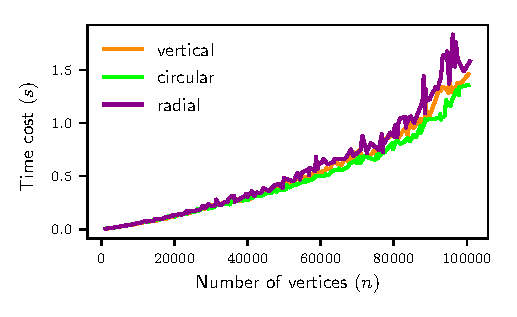
\includegraphics[width=0.5\linewidth]{chapters/sc/fig/runtime.eps}
    \caption{Running time in seconds with respect to environment complexity (number of vertices). }
    \label{fig:sc-simulations_runtime}
\end{figure}

\textbf{Different environment settings.}
Lastly, we evaluate the impact of environmental changes, considering factors including the spatial distribution of polygonal obstacles as well as 
the size distribution of the obstacles. 
%
All in all, three settings are considered: (1) The polygons are regularly distributed 
and are of similar size, (2) the polygons are randomly distributed and are of similar size,
and (3) the polygons are regularly distributed, and their sizes can vary dramatically. 
The first and the third settings are illustrated in the top row of ~\ref{fig:sc-runtime_env}.
%
For these settings, we compare the time it takes to compute solutions for many polygonal
obstacles and also the number of robots required to achieve $80\%$ probabilistic guarantee 
under the exponential decay sensing model.
%
As we can observe, there is little difference as the settings change. 

\begin{figure}[h]
    \centering
    \hspace{5mm}
    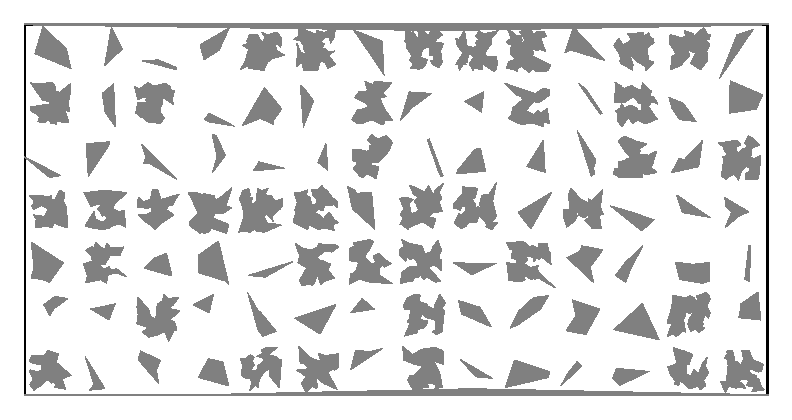
\includegraphics[width = 0.44\linewidth]{chapters/sc/fig/expr_inst_regular.eps}\hspace{1mm}
    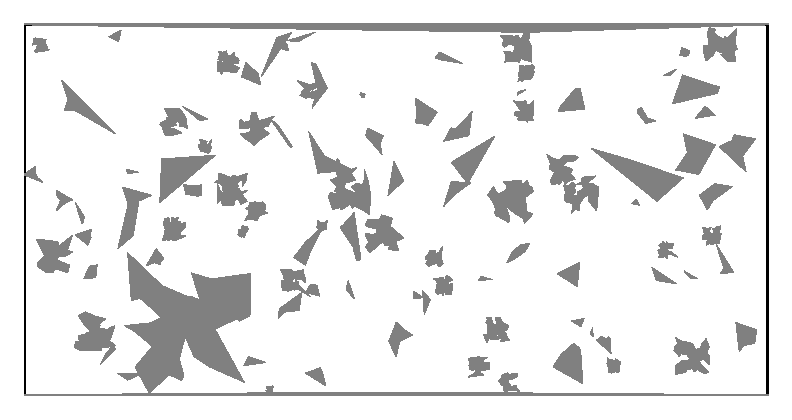
\includegraphics[width = 0.44\linewidth]{chapters/sc/fig/expr_inst_varscale.eps}
    \vspace{3mm}
    
    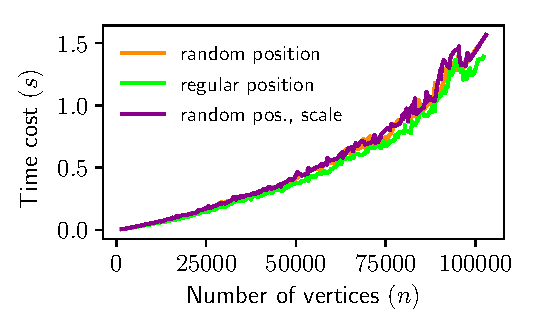
\includegraphics[width=.47\linewidth]{chapters/sc/fig/runtime_env.eps}
    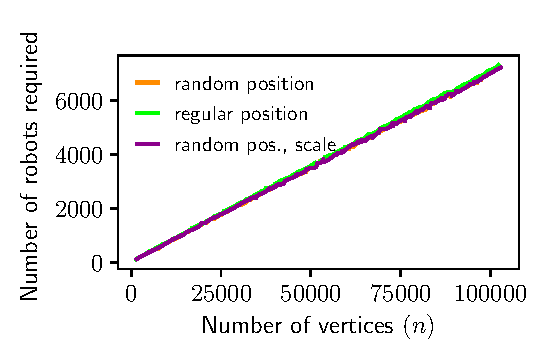
\includegraphics[width=.48\linewidth]{chapters/sc/fig/n_env.eps}
    \caption[Random instance and runtime time]{
    [top] Random instance with regularly distributed obstacles and instance with random obstacle scales and positions.
    [bottom] Running time for different randomly generated environments and the number of robots required for different randomly generated environments.}
    \label{fig:sc-runtime_env}
\end{figure}

%Based on the evaluation, one somewhat interesting conclusion we can draw is 
%that, the solution to the robot allocation task for carrying out pre-determined 
%sweep schedule is fairly ``stable''; it is unlikely to have dramatic 